\section[Inductive Synthesis]{Inductive synthesis of LTS models from MSC and hMSC}

%%%%

\begin{frame}{Inductive LTS synthesis from MSC and hMSC}

  \begin{block}{Research question(s)}
		\begin{itemize}
			\item Scenarios are known to be inherently partial, they only provide typical 
            examples of system the usage
			\item Generalizing observed behaviors looks interesting in practice
      \item How to synthesize LTSs from MSCs while generalizing behaviors?
		\end{itemize}
	\end{block}

  \begin{block}{Outline}
    \begin{itemize}
      \item From grammar induction to model induction
      \item Interactive induction of LTS models from MSCs
      \item Pruning the induction space with state information
      \item Pruning the induction space with goals
      \item Pruning the induction space with control information
    \end{itemize}
	\end{block}

\end{frame}
 
%%%%%
\subsection{From grammar induction to model induction}
\begin{frame}{From grammar induction to behavior model induction}
  \begin{block}{Grammar Induction}
	  \begin{itemize}
	   	\item aims at learning a regular language $L$ from a set of positive and negative strings,
			      i.e. respectively belonging and not belonging to the language
		  \item Also known as \emph{Automaton Induction} when $L$ is represented by a Finite Automaton $A(L)$
	  \end{itemize}
  \end{block}
  \begin{block}{Applicability to LTS Induction}
	  \begin{itemize}
		  \item LTS are DFA with all accepting states, i.e. they define a subclass of regular 
            languages (prefix-closed languages)
		  \item A positive MSC is an accepting trace in the system LTS (obtained by composition of all agent LTS)
		  \item A positive (resp. negative) MSC can be seen as a positive (resp. negative) string of the language accepted 
            by the system LTS
	  \end{itemize}
  \end{block}
\end{frame}

%%%%%

\begin{frame}{Background on Grammar Induction}
  \begin{block}{Overview}
	  \begin{itemize}
	   	\item \emph{Grammar induction} aims at learning a regular language $L$ from a set of positive and negative strings,
			   i.e. respectively belonging and not belonging to the language
		  \item Also known as \emph{Automaton Induction} when $L$ is represented by a (Deterministic) Finite Automaton $A(L)$
	  \end{itemize}
  \end{block}
  \begin{block}{Important results}
	  \begin{itemize}
		  \item RPNI algorithm (Regular Positive and Negative Inference)
		  \item Necessary condition for convergence: \emph{structural completeness} of the sample (each transition and accepting state 
			  of the automaton is used at least once in the input sample)
		  \item Sufficient condition for convergence: the input sample contains a \emph{characteristic sample} for $A(L)$
	  \end{itemize}
  \end{block}
\end{frame}

%%%%%

\begin{frame}{RPNI algorithm}
  From a Prefix Tree Acceptor, accepting the positive sample only, ...
  \begin{center}
	  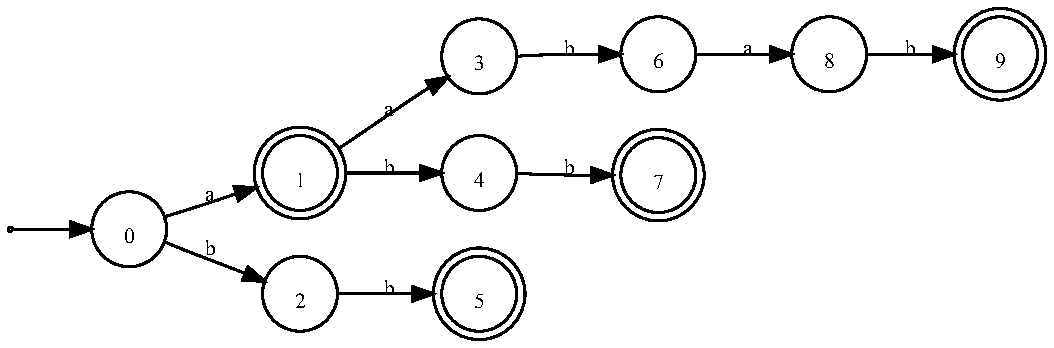
\includegraphics[width=9cm]{images/dfa_merge_0.pdf}
  \end{center}
  ... induce a DFA by successively merging well-chosen state pairs (BlueFringe heuristics), under the control of the negative sample
  \begin{center}
	  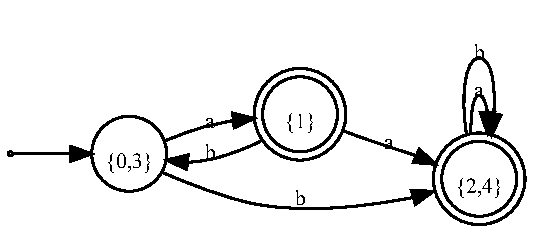
\includegraphics[width=6cm]{images/dfa_merge_3.pdf}
  \end{center}
\end{frame}

%%%%%%
\subsection{Interactive induction of LTS models from MSCs}

\begin{frame}{Grammar Induction for LTS Synthesis: a short summary}
	\begin{block}{Question addressed}
		\begin{itemize}
			\item Importance of negative strings; are they initially available from end-users?
			\item How to ensure consistency with other models?
			\item Assumption that all MSC start in the same system state, what about loops and reuse?
		\end{itemize}
	\end{block}
	\begin{block}{Main results}
		\begin{itemize}
			\item Our interactive variant of RPNI, namely $QSM$, when few negative scenarios are initially provided
			\item Injecting fluent definitions, goals and legacy components ensures inter-model consistency and prunes the process
			\item Other contributed variants, namely $ASM$ and $ASM^*$, support an hMSC as input, relaxing the assumption mentionned
		\end{itemize}
	\end{block}
\end{frame}

\subsection{Interactive LTS Synthesis from MSC}
\begin{frame}{Interactive LTS Synthesis from MSC: the QSM algorithm}
	\begin{block}{Summary}
		\begin{itemize}
			\item RPNI with BlueFringe heuristic for selecting state pairs to merge
			\item When two states are merged, scenario queries are submitted to an end-user for classification as positive or negative behaviors
			\item The end-user, aka Oracle, guides the induction process, avoiding poor generalizations
			\item Query generation relies on the definition of a \emph{characteristic sample}, which provides a convergence criteria
		\end{itemize}
	\end{block}
	\begin{block}{Related publications}
   		\scriptsize
		\begin{itemize}
			\item Damas C., Lambeau B., and van Lamsweerde A, \emph{Generating Annotated Behavior Models From End-User Scenarios},
			     	IEEE Transactions on Software Engineering, Special Issue on Interaction and State-based Modeling, Vol. 31, No. 12, pp. 1056-1073, 2005.
			\item P. Dupont, B. Lambeau, C. Damas, and A. van Lamsweerde, \emph{The QSM Algorithm and its Application to Software Behavior Model Induction},
         		                   Applied Artificial Intelligence, Vol. 22, 2008, 77-115.
		\end{itemize}
	   \end{block}
\end{frame}

\subsection{Pruning the induction space with state information}
\begin{frame}{Pruning the induction with fluents}
	\begin{block}{Summary}
		\begin{itemize}
			\item PTA states can be decorated with fluent values, using the decoration algorithm
			\item The induction process can be constrained to avoid merging non equivalent states
		\end{itemize}
	\end{block}
	\begin{center}
		$fluent\;mov(ing) = <start, \{stop, emergency\;stop\}> initially\;false$
	\end{center}
	\begin{center}
		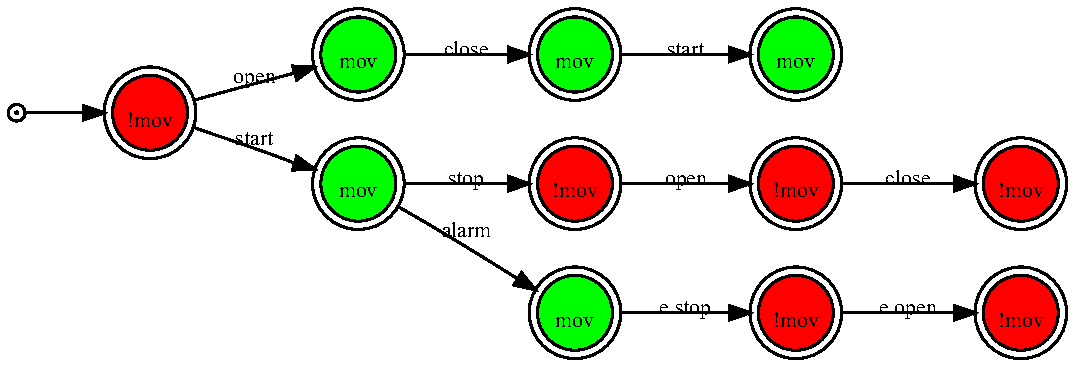
\includegraphics[width=9cm]{images/train_pta.pdf}
	\end{center}
\end{frame}

\subsection{Pruning the induction with goals}
\begin{frame}{Pruning the induction with goals}
	\begin{block}{Summary}
		\begin{itemize}
			\item Color PTA states with corresponding states in the tester. Avoid merging two PTA states not sharing the color
		\end{itemize}
	\end{block}
	\begin{columns}
		\column{.45\textwidth}
			\begin{center}
				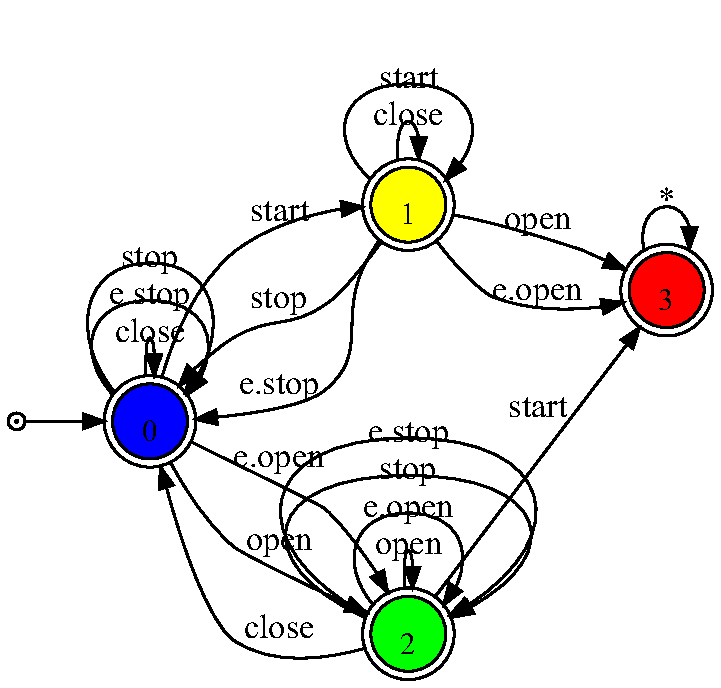
\includegraphics[width=4cm, trim = 0mm 0mm 0mm 10mm, clip]{images/MaintainDoorsClosedWhileMoving_colored.pdf}
			\end{center}
		\column{.45\textwidth}
			\begin{center}
				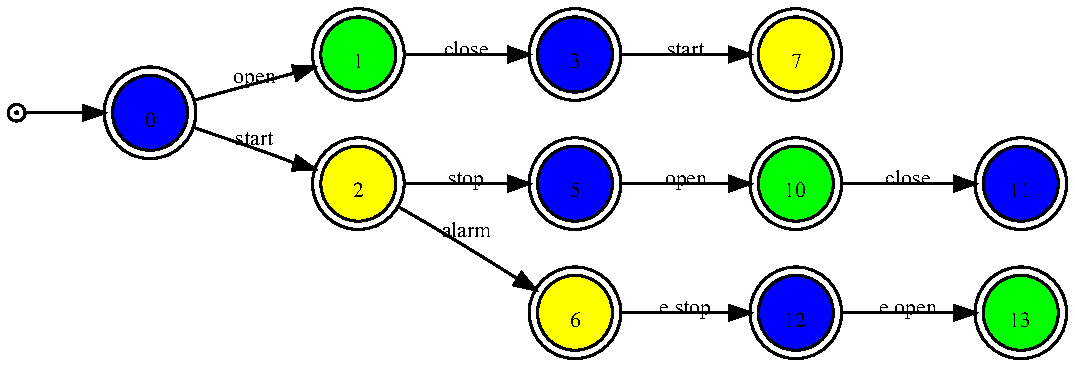
\includegraphics[width=5.5cm, trim = 0mm 0mm 0mm 0mm, clip]{images/train_pta_decorated.pdf}
			\end{center}
	\end{columns}
	\begin{block}{Open questions}
		\begin{itemize}
			\item Sound but too strong! This is related to another open issue on $ASM^*$ about the negative language $L^-$ (see later)
		\end{itemize}
	\end{block}
\end{frame}

\begin{frame}{Pruning the induction though equivalence classes}
	\begin{block}{State coloring as a generalization}
		\begin{itemize}
			\item Equivalence relations can be defined on PTA states and induction process constrained to avoid merging
				non equivalent states.
			\item Legacy components can be used in a similar way, for example
		\end{itemize}
	\end{block}
	\begin{block}{Open questions}
		\begin{itemize}
			\item Defining equivalence classes could be extended in the light of lattice-based decorations
			\item We are convinced that additional architectural constraints could be used (to avoid introducing implied scenarios, for example)
		\end{itemize}
	\end{block}
	\begin{block}{Related publications}
   		\scriptsize
		\begin{itemize}
			\item C. Damas, B. Lambeau and A. van Lamsweerde, \emph{Scenarios, Goals, and State Machines: a Win-Win Partnership for Model Synthesis}, 
                                      Proc. FSE'06: Intl. ACM Symposium on the Foundations of Software Engineering, Portland (OR), November 2006. 
		\end{itemize}
	   \end{block}
\end{frame}

\subsection{Pruning the induction with control information}
\begin{frame}{Pruning the induction with control information}
	\begin{block}{Questions addressed}
		\begin{itemize}
			\item Assumption that all MSCs start in the same initial state
			\item End-users would like to capture loops when known
			\item Would it be possible to take a hMSC as input instead of a collection of MSCs?
		\end{itemize}
	\end{block}
	\begin{block}{Main results}
		\begin{itemize}
			\item Introduction of \emph{mandatory merge constraints} on PTA states, which is the logical counterpart
				of equivalence classes
			\item The $ASM$ algorithm generalizes a positive language $L^+$ under the control of a negative sample $S^-$. 
			          $ASM^*$ generalizes a positive language $L^+$ under the control of a negative language $L^-$
			\item Therefore, behaviors described in a hMSC can be generalized under the control of negative MSCs 
		\end{itemize}
	\end{block}
\end{frame}

\begin{frame}{Pruning the induction with control information}
	\begin{block}{Open questions}
		\begin{itemize}
			\item Three concurrent techniques about pruning with goals: equivalent classes (too strong), $ASM^*$ (looks not 
				applicable directly) and Coste's work in \cite{Coste04}
			\item $ASM$ and $ASM^*$ do not support the BlueFringe heuristics nor the interactive feature
			\item Theoretical GI questions because $ASM$ and $ASM^*$ do not perfectly fit the classical regular language learning framework
		\end{itemize}
	\end{block}
	\begin{block}{Related publications}
   		\scriptsize
		\begin{itemize}
			\item B. Lambeau, C. Damas and P. Dupont, \emph{State-merging DFA Induction Algorithms with Mandatory Merge Constraints}, 
	                             Lecture Notes in Artificial Intelligence No. 5278, Springer, pp. 139-153, 2008, 9th International Colloquium on Grammatical Inference, 
	                             St Malo, France, September 22-24.
			\item No feedback in the RE community so far
		\end{itemize}
	   \end{block}
\end{frame}
